\section{Tagger Performance} 

\frame{
    \frametitle{ Tagger Performance After Retuning }
    \begin{itemize}
    \end{itemize}

    { \small valid1.410000.PowhegPythiaEvtGen\_P2012\_ttbar\_hdamp172p5
    \_nonallhad.digit.AOD.e4993
    \_s3214\_r11234\_d1505\_r11280\_tid17270662\_00 }

    \tiny (Based on JIRA Ticket: https://its.cern.ch/jira/browse/ATR-19472)

    \vfill

    \begin{table}
    \resizebox{\textwidth}{!}{%
    \begin{tabular}{| l | l | l | l |}
        \hline
        Trigger Title & Input Chain & Track Key & Prm Vtx Key \\
        \hline \hline
        HLT & HLT\_j35\_boffperf\_split & InDetTrigTrackingxAODCnv\_Bjet\_IDTrig & xPrimVx\\
        FTK IDTrig & HLT\_j35\_boffperf\_split\_FTK\_L1J15\_FTK & InDetTrigTrackingxAODCnv\_Bjet\_FTK\_IDTrig & PrimVertexFTK\\
        FTK Refit & HLT\_j35\_boffperf\_split\_FTKRefit\_L1J15\_FTK & InDetTrigTrackingxAODCnv\_Bjet\_FTKRefit & PrimVertexFTK\\
        FTK-HLT & HLT\_j35\_boffperf\_split\_FTKVtx\_L1J15\_FTK & InDetTrigTrackingxAODCnv\_Bjet\_IDTrig & PrimVertexFTK\\
        \hline
    \end{tabular}}
    \end{table}

}
\frame{
    \frametitle{ MV2c10 Performance } 
    \begin{figure}
        \includegraphics[width=\linewidth,height=\textheight,keepaspectratio]{btag_c10_score_comparison/performance_roc_ttbar}
    \end{figure}
    \statwarn
}
\frame{
    \frametitle{ IP2D and IP3D Performance } 
    \begin{columns}
        \begin{column}{0.5\textwidth}
            \begin{figure}
                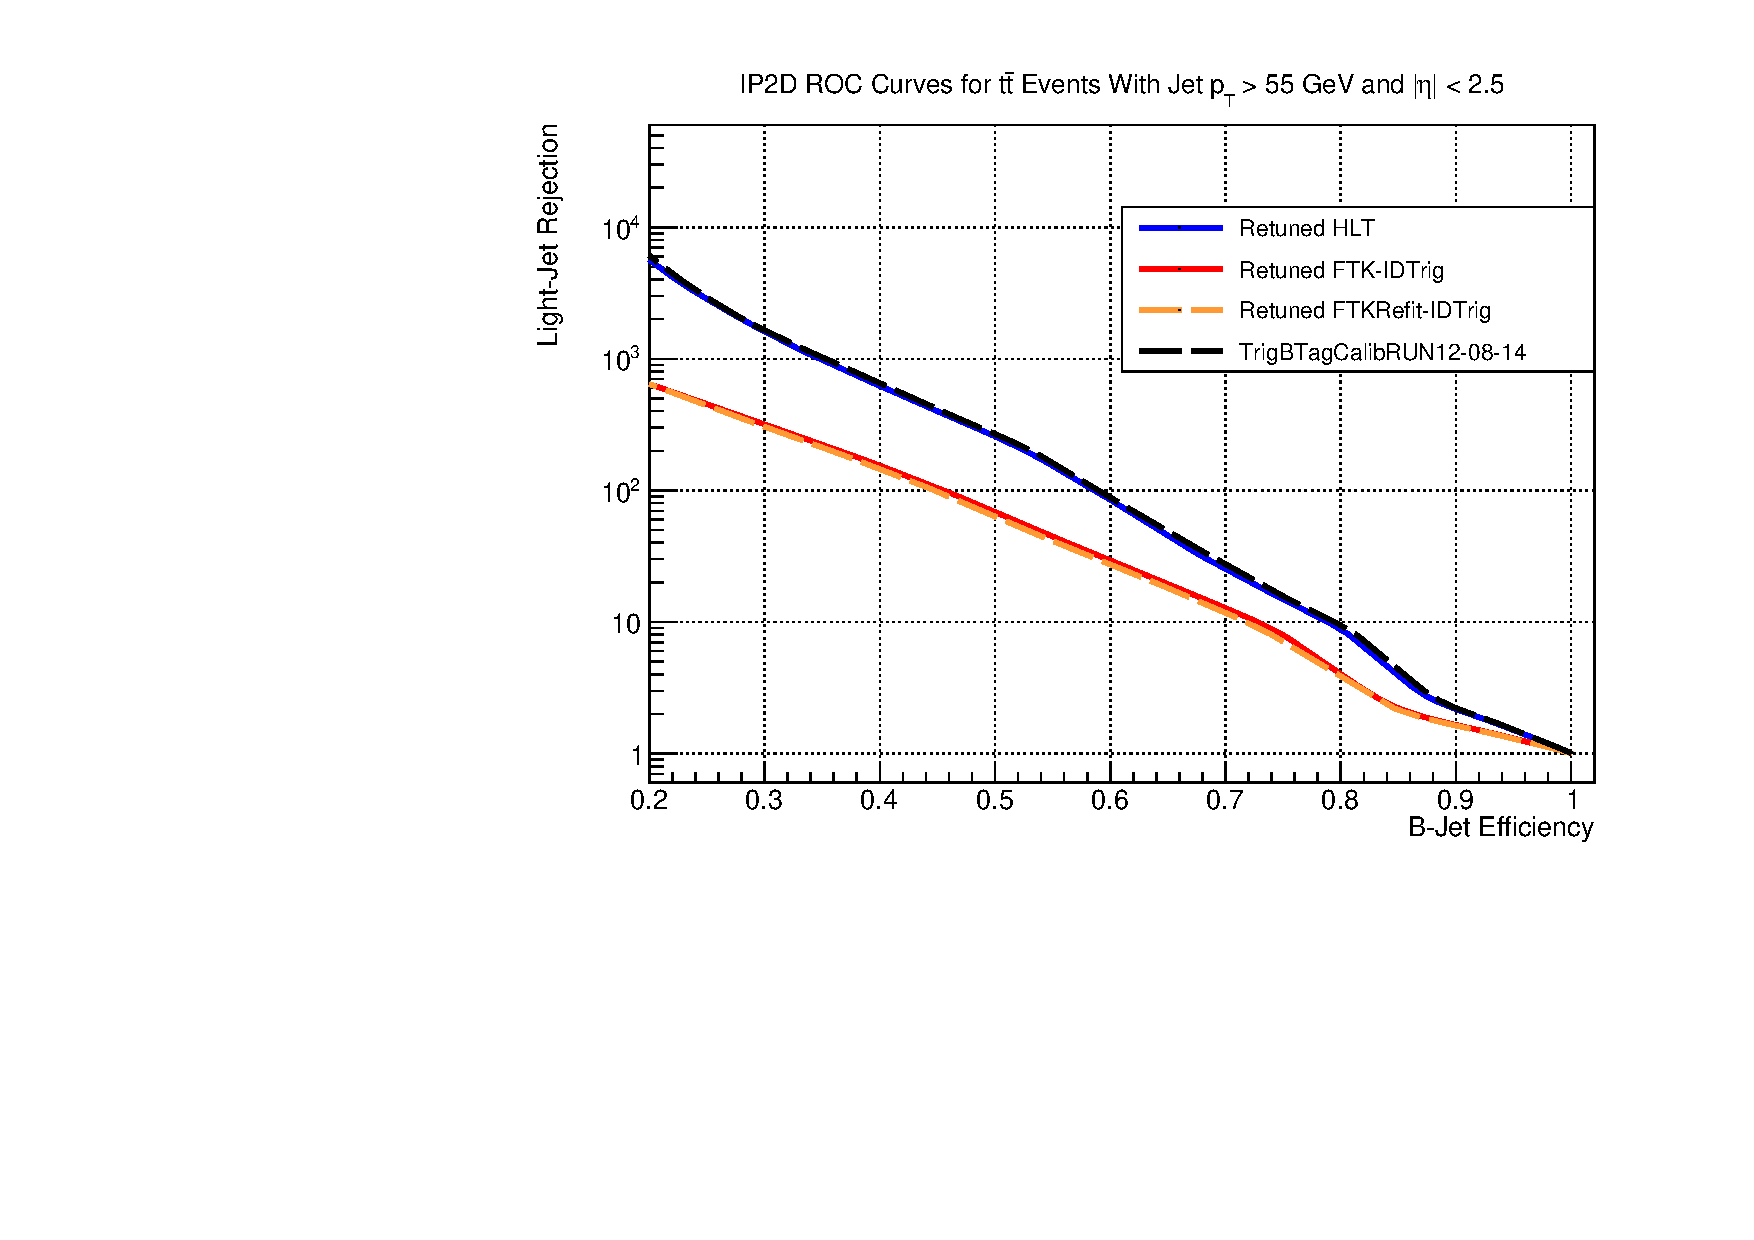
\includegraphics[width=\linewidth,height=\textheight,keepaspectratio]{ipxd_performance/performance_roc_ttbar_ip2d}
            \end{figure}
        \end{column}
        \begin{column}{0.5\textwidth}
            \begin{figure}
                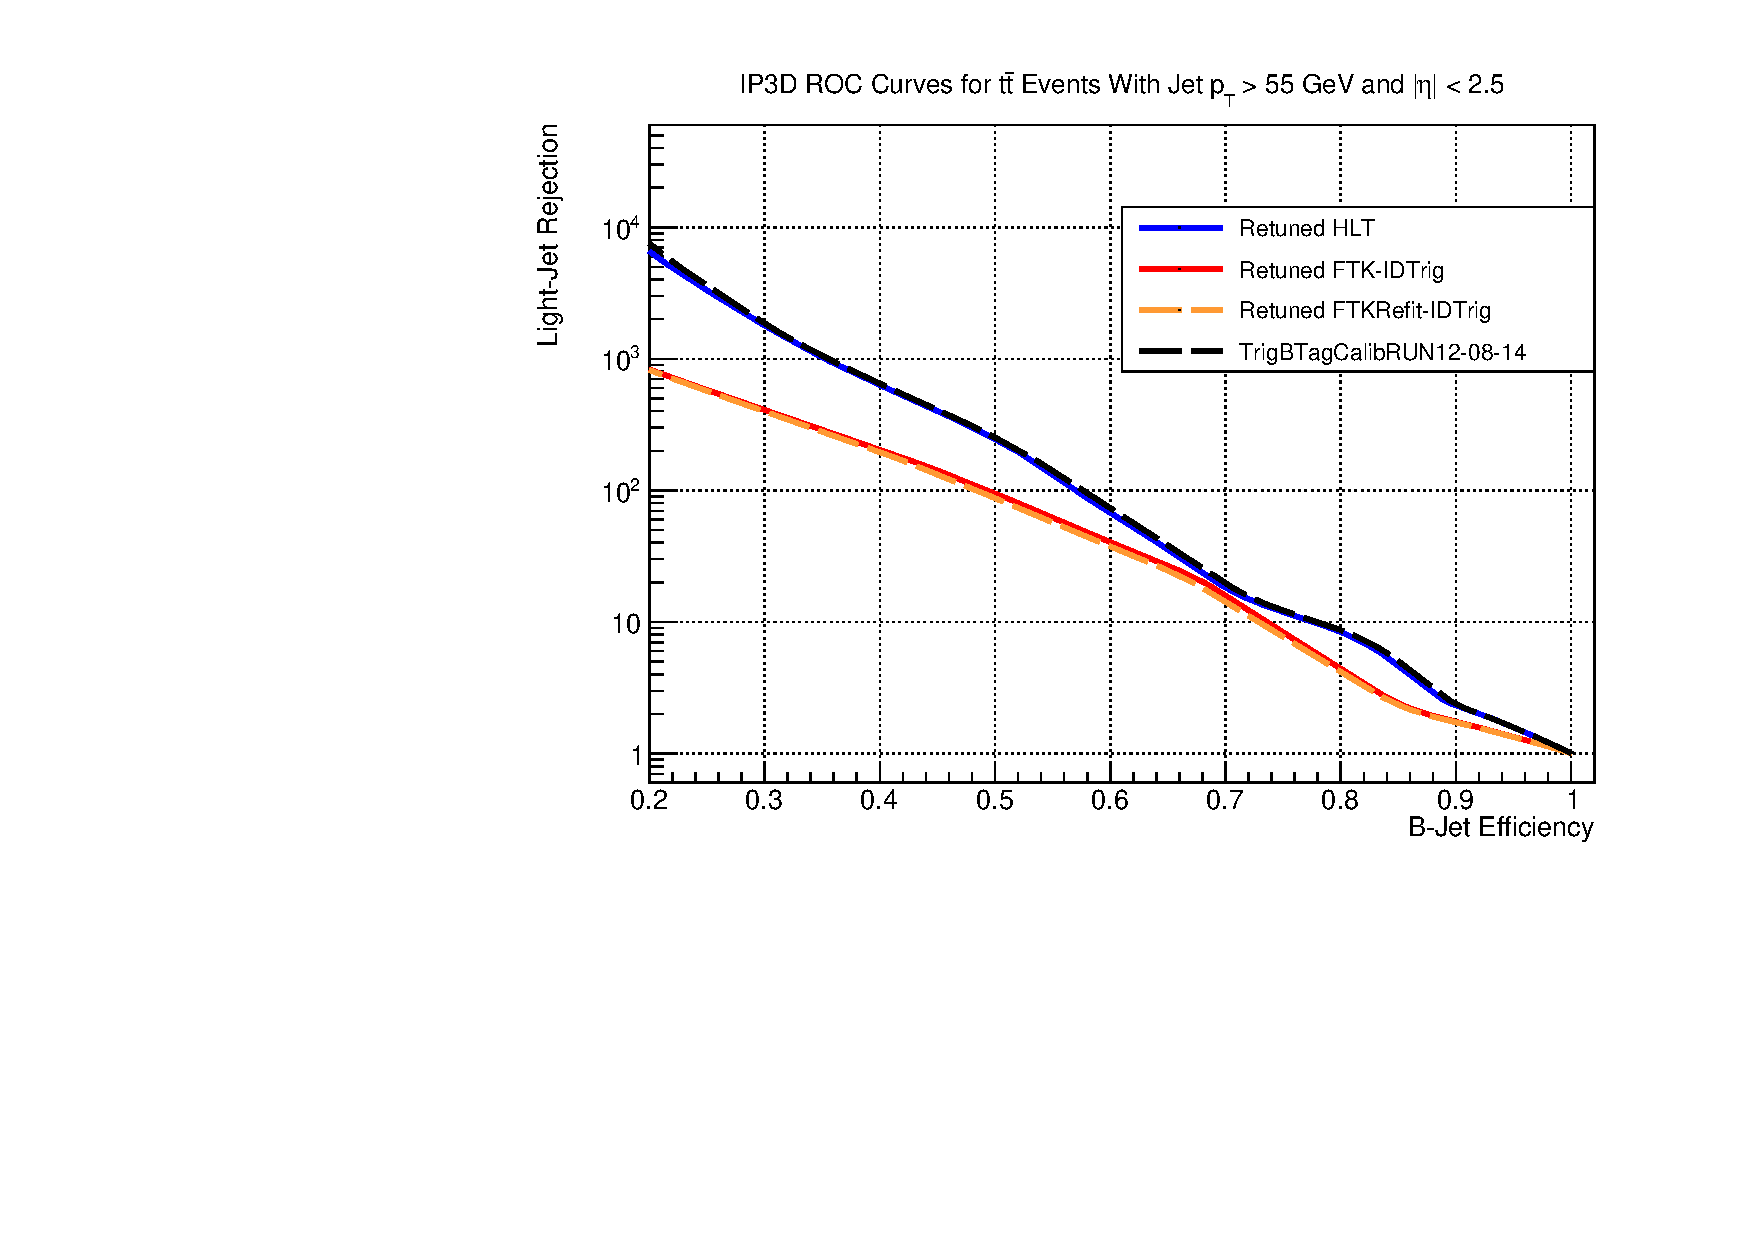
\includegraphics[width=\linewidth,height=\textheight,keepaspectratio]{ipxd_performance/performance_roc_ttbar_ip3d}
            \end{figure}
        \end{column}
    \end{columns}
    \statwarn
}


